\section{Simulation Analysis}
\label{sec:simulation}

\hspace{0,5cm} This section covers the circuit simulation using the Ngspice tool, where the AC/DC converter was simulated for 10 periods using the default diode model.
\par Firstly, the transformer was replaced by an ideal model using an dependent current source and an dependent voltage source. Then, by trial and error the values of the resistors, capacitor and n parameter were adjusted reaching a good accuracy. The goal was to reach the closest value to 12V in the output voltage.
\par As asked in the lab assignment, the input voltage of the the secondary circuit, the output voltage of the envelope detector, the output voltage of the voltage regulator and (v(5)-12) were computed and ploted.
\par Later in this report, we will compare this results with the theoretical ones but for now we will just show them.

The Table~\ref{tab:op1} shows the output voltages results for the circuit described in introduction.

\begin{table}[!ht]
  \centering
  \begin{tabular}{|l|r|}
    \hline    
    {\bf Name} & {\bf Value [A or V]} \\ \hline
    Cost & 123.208\\ \hline
merit & 54.3849\\ \hline

  \end{tabular}
  \caption{Outpu voltages results in Volts}
  \label{tab:ngs1}
\end{table}

The Table~\ref{tab:op2} show the merit value obtained by the group.
\begin{table}[!ht]
  \centering
  \begin{tabular}{|l|r|}
    \hline    
    {\bf Name} & {\bf Value [A or V]} \\ \hline
    V(CE) & 2.78156\\ \hline
V(BE) & 0.70931\\ \hline
V(CE)>V(BE) & Yes\\ \hline

  \end{tabular}
  \caption{Merit values}
  \label{tab:ng2}
\end{table}

\begin{figure}[ht!] \centering
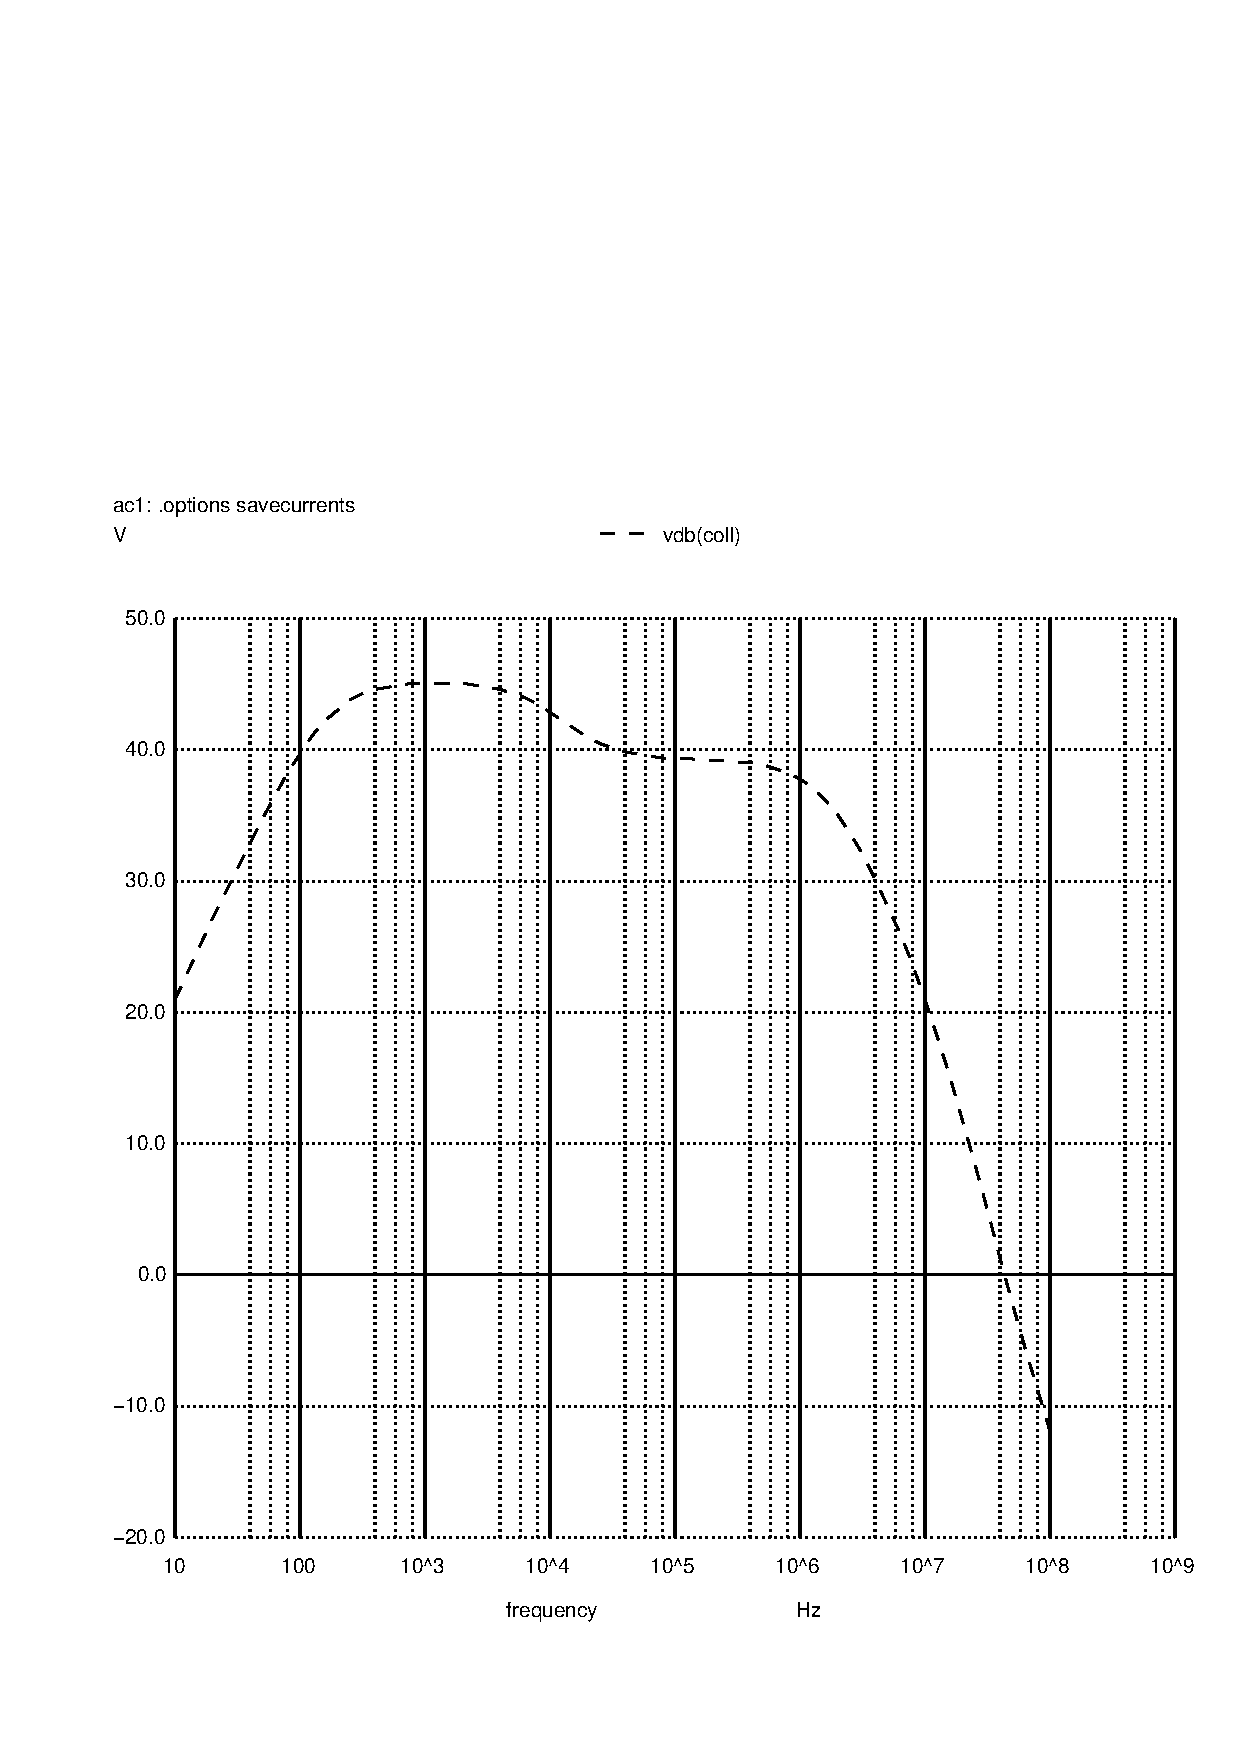
\includegraphics[width=0.5\linewidth]{../sim/vo1f.pdf}
\caption{Output Voltage of the envelope detector v(4)} 
\label{fig:sim1}
\end{figure}

\begin{figure}[ht!] \centering
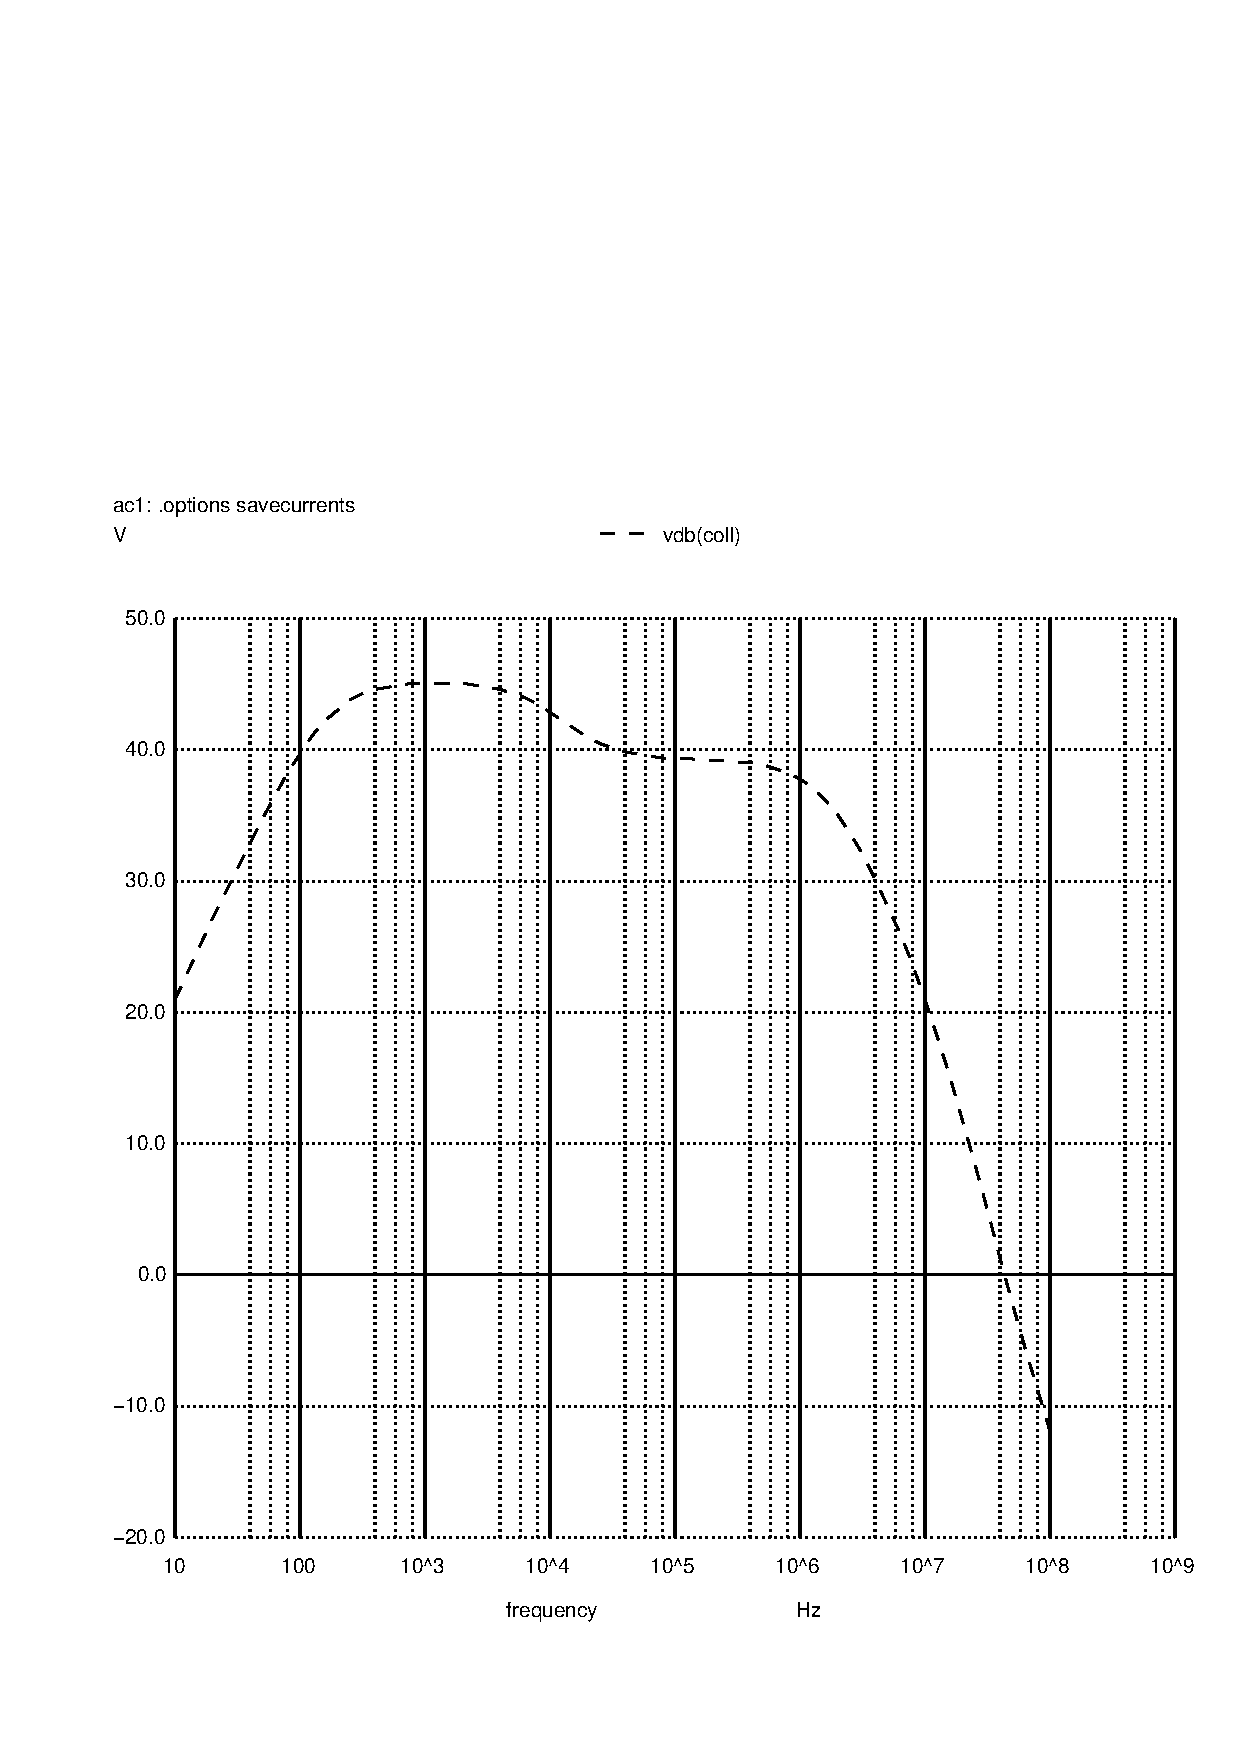
\includegraphics[width=0.5\linewidth]{../sim/vo2f.pdf}
\caption{Input Voltage of the secondary circuit (v(2)-v(3))} 
\label{fig:sim2}
\end{figure}

The Table~\ref{tab:op2} show the merit value obtained by the group.
\begin{table}[!ht]
  \centering
  \begin{tabular}{|l|r|}
    \hline    
    {\bf Name} & {\bf Value [A or V]} \\ \hline
    V(EC) & 4.49605\\ \hline
V(EB) & 0.817257\\ \hline
V(EC)>V(EB) & Yes\\ \hline

  \end{tabular}
  \caption{Merit values}
  \label{tab:ng3}
\end{table}


The Table~\ref{tab:op2} show the merit value obtained by the group.
\begin{table}[!ht]
  \centering
  \begin{tabular}{|l|r|}
    \hline    
    {\bf Name} & {\bf Value [A or V]} \\ \hline
    V_Gain&37.9181\\ \hline
Bandwidth&1.55393E+06\\ \hline
CO_Freq& 8793.49\\ \hline

  \end{tabular}
  \caption{Merit values}
  \label{tab:ng4}
\end{table}


The Table~\ref{tab:op2} show the merit value obtained by the group.
\begin{table}[!ht]
  \centering
  \begin{tabular}{|l|r|}
    \hline    
    {\bf Name} & {\bf Value [A or V]} \\ \hline
    Zin & -548.062 + 82.7641 j\\ \hline

  \end{tabular}
  \caption{Merit values}
  \label{tab:ng5}
\end{table}


